% This LaTeX was auto-generated from MATLAB code.
% To make changes, update the MATLAB code and export to LaTeX again.

\documentclass{article}

\usepackage[utf8]{inputenc}
\usepackage[T1]{fontenc}
\usepackage{lmodern}
\usepackage{graphicx}
\usepackage{color}
\usepackage{hyperref}
\usepackage{amsmath}
\usepackage{amsfonts}
\usepackage{epstopdf}
\usepackage[table]{xcolor}
\usepackage{matlab}

\sloppy
\epstopdfsetup{outdir=./}
\graphicspath{ {./Results_images/} }

\begin{document}



\vspace{1em}

\begin{par}
\begin{flushleft}
Results 1.1: Car path for constraint scheme, 
\end{flushleft}
\end{par}

\begin{par}
\begin{flushleft}
Results 1.2 yRef vs X
\end{flushleft}
\end{par}

\begin{par}
\begin{flushleft}
scheme A
\end{flushleft}
\end{par}

\begin{center}
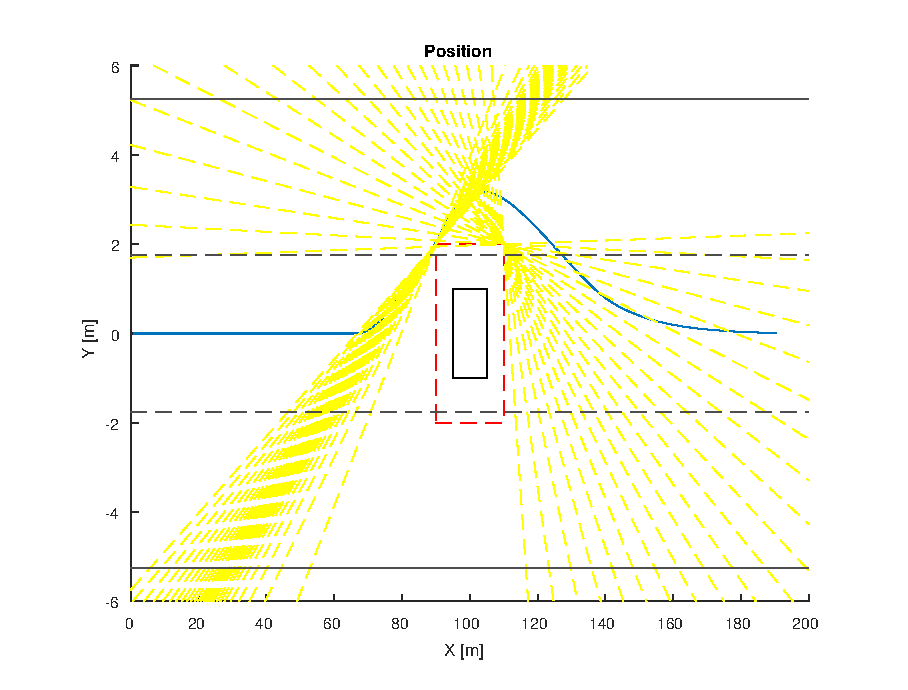
\includegraphics[width=\maxwidth{56.196688409433015em}]{figure_0.eps}
\end{center}
\begin{par}
\begin{flushleft}
Results 1.2: Comparison between both tracking schemes
\end{flushleft}
\end{par}

\begin{center}
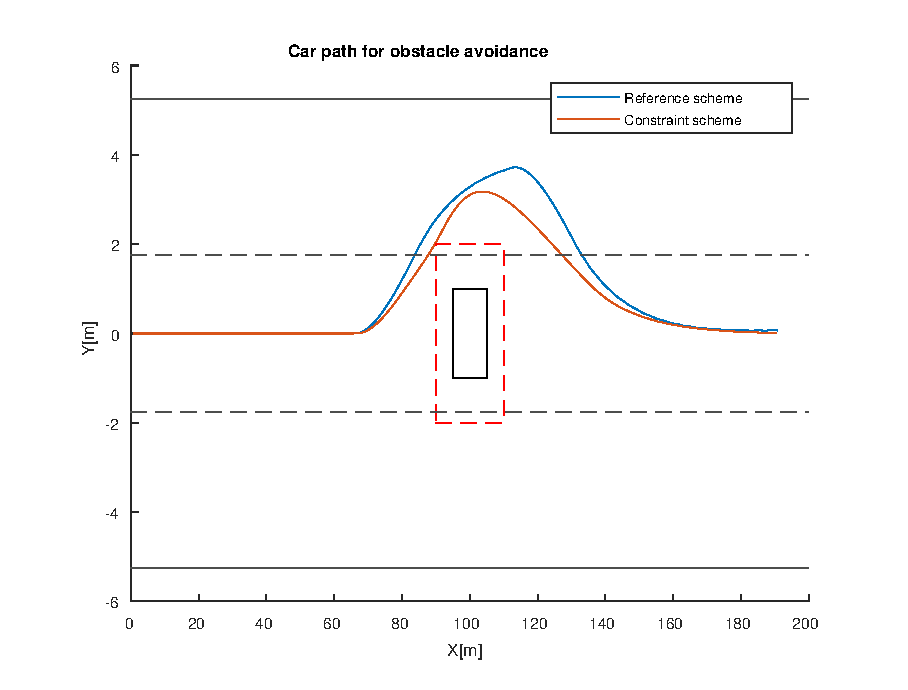
\includegraphics[width=\maxwidth{56.196688409433015em}]{figure_1.eps}
\end{center}

\begin{par}
\begin{flushleft}
Results 1.3: State and input evolution for both schemes (Detection toevoegen)
\end{flushleft}
\end{par}

\begin{center}
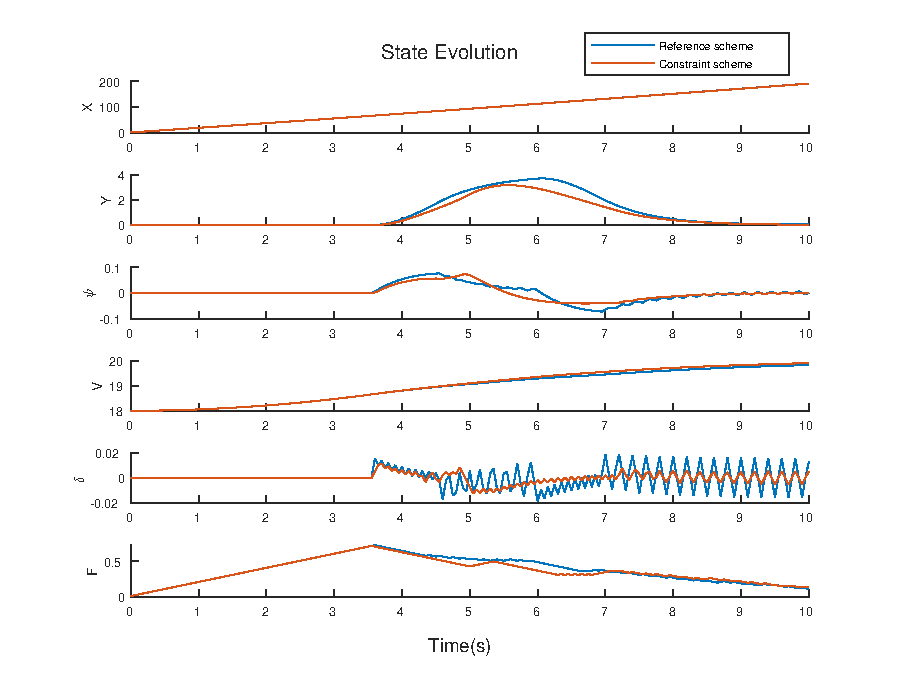
\includegraphics[width=\maxwidth{56.196688409433015em}]{figure_2.eps}
\end{center}

\begin{par}
\begin{flushleft}
Results 1.4: MPC cost for both schemes
\end{flushleft}
\end{par}

\begin{center}
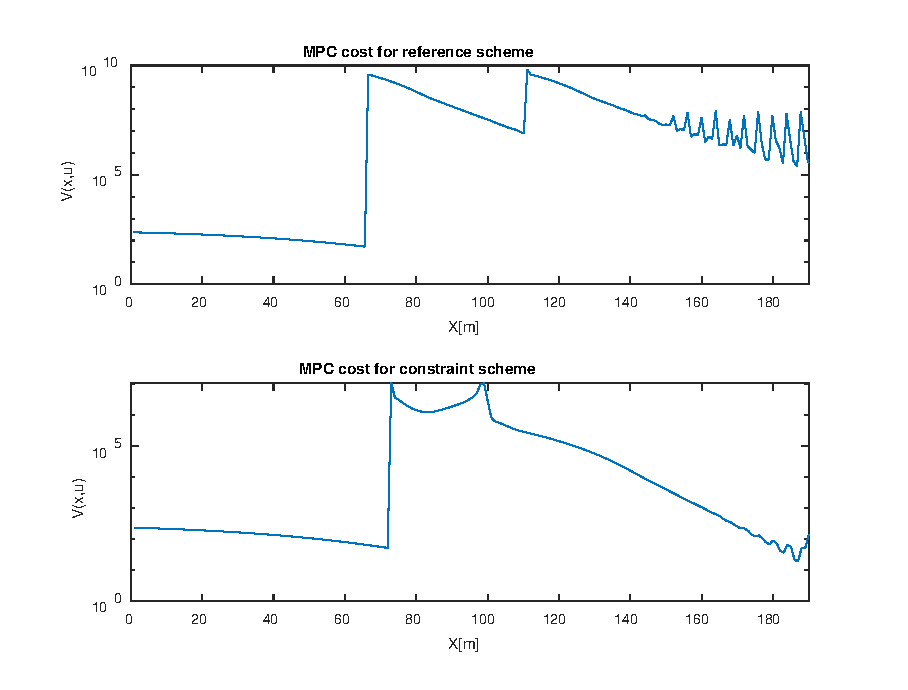
\includegraphics[width=\maxwidth{56.196688409433015em}]{figure_3.eps}
\end{center}

\begin{par}
\begin{flushleft}
Results 2: plots for varying control horizons
\end{flushleft}
\end{par}

\begin{center}
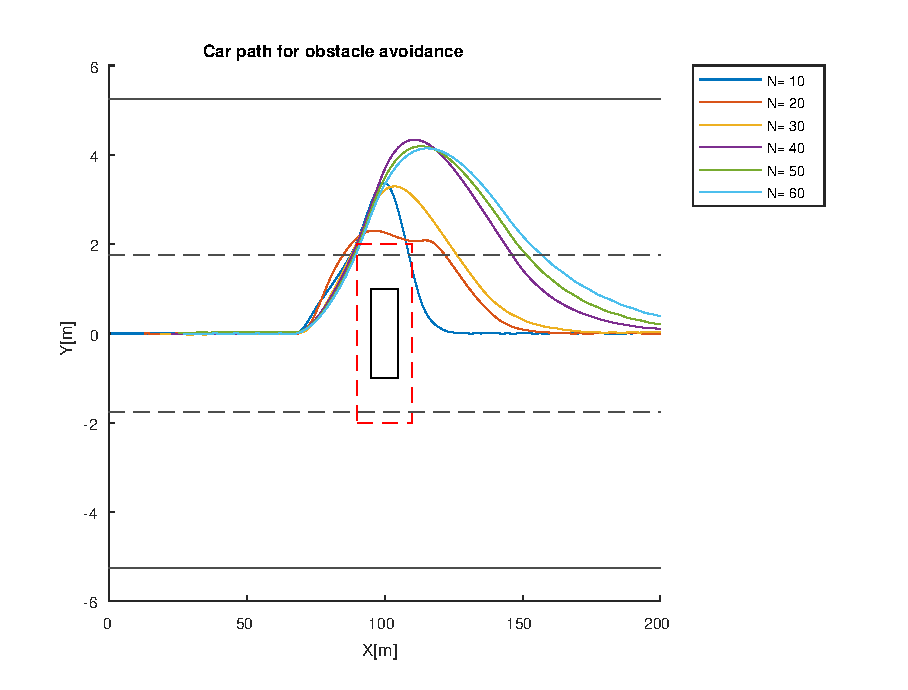
\includegraphics[width=\maxwidth{56.196688409433015em}]{figure_4.eps}
\end{center}
\end{document}
